\section{Sovereign Cloud Stack}
\label{sec:gaia-x-einbettung:scs}

\begin{figure}[h]
  \makebox[\textwidth][c]{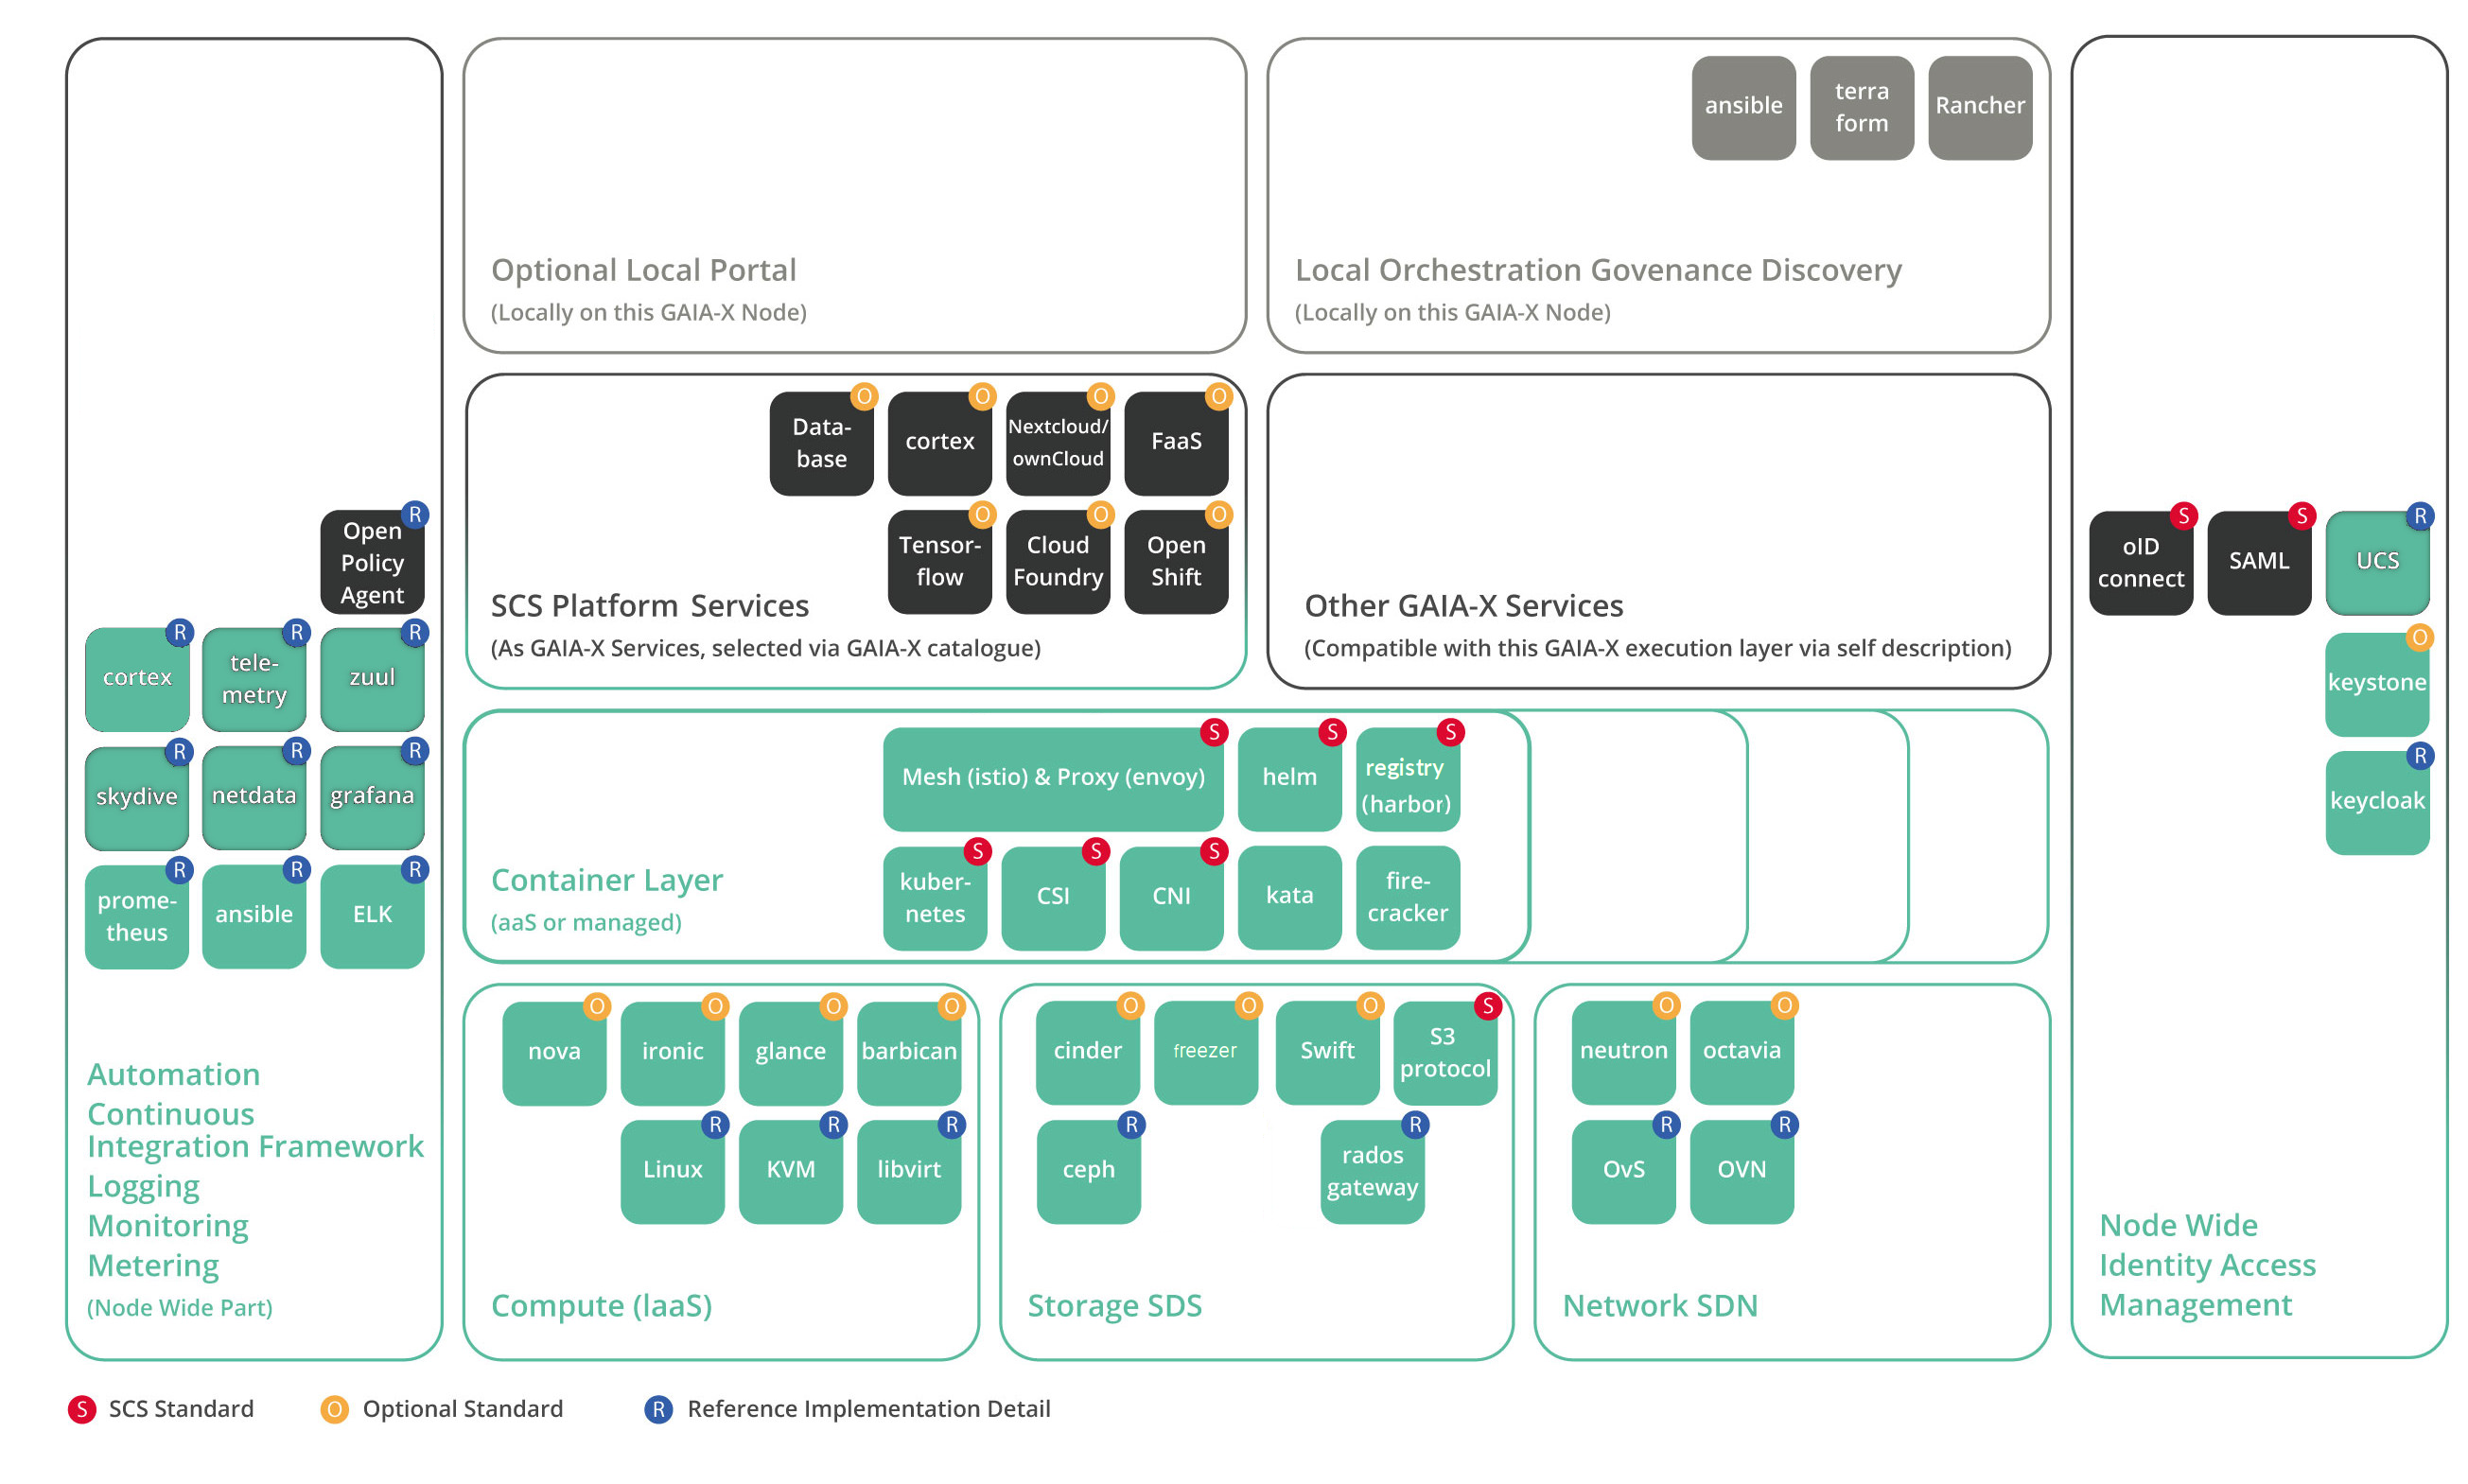
\includegraphics[height=0.85\textwidth]{gfx/chapters/4_gaia-X/scs_architecture.png}}
  \raggedleft
  \caption{Architektur und Komponenten des Sovereign Cloud Stacks}
  \source{\cite{scs}}
  \label{fig:scs_architecture}
\end{figure}

\ac{SCS} ist eine freier Softwarestack zur Erstellung einer standardisierte und souveräne Plattform.
Diese Plattform soll von existierenden und zukünfitgen Cloudprovidern genutzt werden, um eine Gaia-X konforme Infrastruktur zu bieten \cite{scs}.
Ziel des Stacks ist ein Netzwerk von Anbietern, welche durch Nutzung von freier Software und gemeinsamer Standards,
eine interoperable, unabhängige Cloud schaffen \cite{Kagermann2021}.
Als technologischer Standpunkt dient \ref{fig:scs_architecture}, welches die geplante Architektur des \ac{SCS} zeigt. 
Grundlage des Stacks sind OpenStack Services, welche als Projekt für Cloud-Computing Architekturen entwickelt wurden.
Unterteilt wird dies in drei grundlegende Bausteine: \textbf{Compute}, \textbf{Network} und \textbf{Storage},
welche als \ac{IaaS} Services definiert sind.
Die Openstack Services sollen als starke, multitenant fähige Basis für Kubernetes Cluster dienen. 
Der Hauptdienst soll Kubernetes as a Service darstellen, auf dem Provider intern ihre \ac{SaaS} aufbauen können \cite{scs}.
Darauf aufbauend wird ein Container Layer erstellt, welcher mit Hilfe von Containerlaufzeitumgebungen
wie Docker oder 
Podman\footnote{\citeurl{podman}}
gesteuert werden soll \cite{scs}.

Services, wie der in dieser Thesis entwickelte Chat \ac{SaaS}, finden sich auf der übergeordneten Ebene \textbf{SCS Platform Services} wieder.
Für die Entwicklung des Rocket.Chat \ac{SaaS} wurde diese Architektur als Grundbild genutzt, indem 
genannte Technologien des Stacks in der Implementierung berücksichtigt wurden.